\documentclass[a4paper,twoside, onecolumn]{article}
\usepackage[utf8]{inputenc}
\usepackage[T1]{fontenc}
\usepackage[top=3cm, bottom=2cm, left=3cm, right=3cm, marginparwidth=1.75cm]{geometry}
\usepackage{xcolor}
\usepackage{csquotes}%
\usepackage{graphicx}%
\usepackage{caption}%
\usepackage{subcaption}%
\usepackage{amsmath}%
\usepackage[
colorlinks=true,
urlcolor=purple!50!red,
citecolor=blue
]{hyperref}
\usepackage{verbatim}
\usepackage{array} %required for decimal alignment in tables%
\usepackage{siunitx} %required for decimal alignment in tables%

%%% packages

\usepackage{csvsimple}%
\usepackage{lineno}
\linenumbers
\newcommand{\afb}{\mathrm{afb}}
\newcommand{\mic}{\mathrm{mic}}
\newcommand{\mol}{\mathrm{mol}}
%\newcommand{\logplus}{\mathrm{log1}}
\newcommand{\Div}{\mathrm{D}}
\renewcommand{\P}{\mathrm{P}}
\newcommand{\Birth}{\mathrm{Birth}}
\newcommand{\total}{\mathrm{total}}
\bibliographystyle{vancouver}

%opening
\title{Predicting Ebola virus disease risk and the role of African bat birthing}

\author{%%%% Author details
	C. Reed Hranac$^{1}$, Jonathan C. Marshall$^{2}$, Ara Monadjem$^{3, 4}$ and David T.S. Hayman$^{1}$}

\begin{document}
	
	\maketitle
	\begin{center}
		\textbf{Address}
		$^{1}$Molecular Epidemiology and Public Health Laboratory, Hopkirk Research Institute, Massey University, Private Bag, 11 222, Palmerston North 4442, New Zealand\\
		$^{2}$Institute of Fundamental Sciences Massey University, Private Bag 11 222, Palmerston North 4442, New Zealand\\
		$^{3}$Department of Biological Sciences, University of Eswatini, Private Bag 4, Kwaluseni, Eswatini\\
		$^{4}$Mammal Research Institute, Department of Zoology and Entomology, University of Pretoria, Pretoria, South Africa
	\end{center}
	\subsubsection*{Corresponding Authors}
	C. Reed Hranac\\
	c.r.hranac@massey.ac.nz\\
	David T.S. Hayman\\
	d.t.s.hayman@massey.ac.nz\\
	\newpage\clearpage
	
	\subsubsection*{Keywords}
	Ebolavirus $|$ Chiroptera $|$ Pteropodidae $|$ Spillover $|$ Viral Ecology $|$ Spatio-temporal Poisson point process $|$ Ecological niche model
	
	\begin{abstract} %%213 words
		Ebola virus disease (EVD) presents a threat to public health throughout equatorial Africa. Despite numerous 'spillover' events into humans and apes, the maintenance reservoirs and mechanism of spillover are poorly understood. Evidence suggests fruit bats play a role in both instances, yet data remain sparse and bats exhibit a wide range of life history traits. Here we pool sparse data and use a mechanistic approach to examine how birthing cycles of African fruit bats, molossid bats, and non-molossid microbats inform the spatio-temporal occurrence of EVD spillover. We create ensemble niche models to predict spatio-temporally varying bat birthing and model outbreaks as spatio-temporal Poisson point processes. We predict three distinct annual birthing patterns among African bats along a latitudinal gradient. Of the EVD spillover models tested, the best by quasi-Akaike information criterion (qAIC) and by out of sample prediction included significant African bat birth-related terms. Temporal bat birthing terms fit in the best models for both human and animal outbreaks were consistent with hypothesized viral dynamics in bat populations, but purely spatial models also performed well. Our best model predicted risk of EVD spillover at locations of the 2018 EVD outbreaks in the Democratic Republic of the Congo was within the top 12-35\% and 0.1\% of all $25\times25$km spatial cells analyzed in sub-Saharan Africa. Results suggest that sparse data can be leveraged to help understand complex systems.
		
	\end{abstract}
	
	\section*{Introduction:}
	Since the first reports of Ebola virus disease (EVD) in the late 1970s outbreaks have occurred sporadically \cite{Pourrut2005}, with 34 identified human index cases to date (Fig.~\ref{fig:F1}). The 2013--2016 West African EVD epidemic caused the death of at least 11,310 people and was a Public Health Emergency of International Concern \cite{Briand2014}. Outbreaks have been unpredictable, sometimes including more than one primary transmission or ‘spillover’ event, and together with high case fatality rates cause significant strain on public health authorities in typically resource poor settings \cite{Pigott2016}. Additional conservation concerns have arisen such as the large scale great ape die-offs linked to EVD in central Africa \cite{Leroy2004}. Despite decades of research the ecology, sylvatic maintenance, and mechanisms of spillover of these viruses to humans, or non-humans, have remained undetermined \cite{Olival2014}.\par
	\begin{figure}[h!]
		\centering
		\includegraphics[width=.95\linewidth]{Fig1DRCUpdate.eps}
		\caption{\textbf{Spatial and temporal detection of ebolavirus by host taxonomic group.} \textit{Top left:} Location of all EVD index spillover events and detections within bat populations. Zoom panel focuses in on the border of Gabon and Republic of Congo. \textit{Bottom left:} Viral detection by taxonomic classes (non-human timeline grey points are human events for reference). \textit{Right:} Frequency of viral detection by taxonomic host collapsed into a single year and aggregated by month. Bats are orange, chimpanzees black, duikers green, gorillas blue, rodents purple and humans red. In all cases except for the bats detections represent unique spillover events. For bats, a detection represents the recovery of an ebolavirus viral RNA gene fragment. The two most recent outbreaks in the DRC are denoted in gold. All references, are available within the online material.}
		\label{fig:F1}
	\end{figure}
	The genus \textit{Ebolavirus} (family \textit{Filoviridae}) is composed of five recognized viral species, four of which are agents of EVD \cite{Olival2014}. An additional proposed sixth \textit{Ebolavirus} species with unknown ability to cause EVD was also described recently \cite{Goldstein2018}. For the four \textit{Ebolavirus} species known to cause EVD mounting evidence implicates African Old World fruit bat species (Order Chiroptera; family Pteropodidae) as potential reservoirs as defined by Haydon \textit{et al.} \cite{Haydon2002} in maintaining and propagating infection on the landscape \cite{DeNys2018, Leroy2005, Han2016, Pourrut2009}. However, different bats may play roles as both necessary and sufficient hosts in reservoir host communities \cite{nishiura2009find}.	
	To date no full EVD-causing \textit{Ebolavirus} has been isolated from a bat host. Possible reasons for this, if they are true maintenance reservoir hosts, include: the remote geographic locations of the EVD outbreaks; nomadic or migratory nature of bats \cite{Nowak1994}; potentially acute viremic periods \cite{Swanepoel1996}; spatio-temporal extinction and recolonization dynamics, the unknown role of viral persistence and intermittent viral shedding \cite{Schuh2017}, and possibly biased samples unrepresentative of true bat diversity \cite{Leendertz2016}.\par 
	Despite these limitations, RNA viral fragments of ebolaviruses causing EVD have been recovered from three African fruit bat species: Franquet's epauletted fruit bat (\textit{Epomops franqueti}), the Hammer-headed bat (\textit{Hypsignathus monstrosus}), and the Little collared fruit bat (\textit{Myonycteris torquata}) \cite{Leroy2005}. \textit{Ebolavirus} fragments were also detected in four rodent species: two \textit{Praomys sp.}, two \textit{Mus sp.} and one shrew \textit{Sylvisorex ollula} (family: Soricidae)\cite{Morvan1999}, although there is some contention whether these species could effectively act as reservoir hosts \cite{Swanepoel1996} and whether these were in fact active infections \cite{Taylor2010}. Phylogenetic analyses have also suggested that fruit bats have played some role in the recent evolutionary history of \textit{Zaire ebolavirus} \cite{Walsh2005,Biek2006}. Most recently 20\% of an \textit{Ebolavirus} has reportedly been sequenced from an insectivorous greater long-fingered bat (\textit{Miniopterus inflatus}), captured in 2016 in Liberia \cite{Kupferschmidt2019}.\par
	Much of what is postulated about the ecological niche and sylvatic maintenance of ebolaviruses is inferred from a member of its sister genus, \textit{Marburgvirus marburgvirus} (MARV). MARV circulates within cave dwelling Egyptian fruit bat (\textit{Rousettus aegyptiacus}) colonies with seasonal increases in viral shedding among juvenile bats and the high birthing synchrony \cite{Amman2012} although the inclusion of persistent infection with intermittent viral shedding has still to be explored for ebolaviruses. Anti-marburgvirus antibodies have also been detected within co-roosting insectivorous bats, which to date play an unknown role in sylvatic maintenance. Machine learning and infection dynamic simulations have both identified biannual, synchronous birth-pulses as potentially important host life history traits for filovirus maintenance, all traits found within African bat species \cite{Han2016,Hayman2015}.\par
	While there are many similarities between MARV and ebolavirus systems, the principal suspected ebolavirus reservoirs are primarily tree roosting species with far lower colony densities compared to the Egyptian fruit bat. The sporadic occurrence of outbreaks, lifestyles of putative reservoirs, viral dynamics and subsequent antibody production in bats \cite{Swanepoel1996} suggest a potential reliance on meta-populations within a larger reservoir community to sustain sylvatic ebolavirus transmission \cite{Brown2013, Grenfell2001, Han2016, Hassanin2016}. Strong, spatially asynchronous seasonal forcing events, including birthing, likely add additional layers of complexity in disease outbreak events \cite{Duke-Sylvester2011}.\par
	Spatial risk models have previously identified regions of realized and unrealized risk throughout equatorial sub-Saharan Africa, linked to a variety of drivers, including forest fragmentation and vegetation index \cite{Rulli2017,Pigott2014, Pigott2016}. Additional temporal risk models have suggested that EVD spillover risk across the region is greatest during transitions between wet and dry seasons \cite{Schmidt2017}, periods also associated with African bat species birthing events \cite{Cumming1997}. One hypothesis of filovirus spillover risk posits that synchronous shifts in population demographics may be responsible for periods of increased viral shedding similar to those witnessed in the MARV system \cite{Hayman2015, Pourrut2009}.\par 
	In this work we test the hypothesis that birthing among some African bat species is linked to EVD spillover events to humans and forest dwelling animals susceptible to EVD, hereafter referred to as "non-human spillover hosts." Due to the rarity of EVD outbreak events we were not able to model each EVD-causing \textit{Ebolavirus} species separately, and therefore combined them all together to represent a single, general, "ebolavirus" capable of infecting, and causing EVD in mammalian hosts. We created two general model frameworks: a model describing the birthing patterns of African bats; and another to describe the relative spillover risk. We assumed bats were reservoir hosts and that non-human spillover hosts have different habitat use, risk factors and contact patterns with the potential reservoir host(s) than humans. Subsequently we modeled spillover into non-human spillover hosts independently of humans. We then used the two most recent outbreaks of EVD in the Democratic Republic of the Congo (DRC) \cite{Barry2018, WHO2018}, which were excluded from our modeling procedures (but see methods), to test the predictive power of our generated models. \par
	\begin{figure}[h!]
		\centering
		\includegraphics[width=.95\linewidth]{Fig2Complete.eps}
		\caption{\textbf{Spatial and temporal occurrence of bat birthing records obtained from the literature.}
			All results from mainland sub-Saharan Africa for the date and location of bat birth events. African fruit bat species are in green, molossid species in blue, and non-molossid microbats in orange. The gray background represents the study region and regions in white were excluded from this analysis. \textit{Left:} Spatial locations of recorded observations. \textit{Right:} Number of birthing observations in the literature by taxonomic group collapsed into a single year and aggregated by month.}
		\label{fig:F2}
	\end{figure}
	%%
	\section*{Materials and Methods}
	Evolutionary, environmental, and phenological processes undoubtedly drive the timing and location of bat breeding and birthing, yet these intricacies have yet to be fully described. Sparse data exist for the timing bat births, especially in mainland tropical Africa \cite{Cumming1997,Monadjem2010}. To circumvent these issues we compiled the better part of 50 years of ecological research into a single, recirculating year of spatio-temporally defined bat birthing events (full data mining methods in SI Methods). Bat species were subset into three groups: African fruit bats (family Pteropodidae), molossid bats (family Molossidae), and non-molossid microbats, as described by Cumming and Bernard \cite{Cumming1997}. These taxonomic clusters tend to share key life history traits such as diet and reproductive strategies making them useful subgroups for this analysis. Combining these occurrence data with static and temporally explicit geographic covariate layers (see SI Table 2) allowed us to construct temporally defined ecological niche models (ENMs) of bat birthing across a subset of sub-Saharan Africa. This subset was restricted to locations in mainland Africa receiving more than 500mL of precipitation annually, as suggested by Schmidt \textit{et al.} 2017 \cite{Schmidt2017}. While outbreaks have not been observed in much of this region and hypothesized reservoir species use subsets of these regions making them a potentially unrealized viral niche. Unlike most ENMs that correlate a probably of occurrence with environmental conditions at any given location, we modified our procedure to correlate dynamic phenological signals focused on changing environments with bat birthing cycles (see full details for covariate selection and processing in SI methods and SI Table 2). We used a sliding two month observation window to estimate the probability of wild species giving birth across space and time for all pairs of consecutive months where sufficient data existed (see full ENM description in SI Methods).\par
	The ENM results were used and combined with bat diversity in a number of different ways. First and most intuitively, the probability of birthing for the three different taxonomic class were used as covariates where probability of birth occurrence is $P_{T,i,t}$ for each taxonomic group $T$, at location $i$ and time $t$. Next the ENM results were combined with local species diversity estimates to create a ``force of birthing'' ($\lambda_{T,i,t}$) metric, representing the relative number of taxon member species giving birth at any time and space, as defined by:
	\[
	\lambda_{T,i,t} = P_{T,i,t}\Div_{T,i}
	\]
	 where the number of taxonomic members is given by $\Div_{T,i}$. The abbreviations ${afb, mic}$ and ${mol}$ were used to represent African fruit bats, non-molossid microbats, and molossid bats respectively. Third, the total conditional probability $P_{total,i,t}$ of any bat birthing from any of the three taxonomic groups at location $i$ and time $t$, assuming independence, defined by:
	\[
	P_{total,i,t} = 1-\prod\nolimits_{T = 1}^{n} (1-P_{T,i,t})
	\]
	A total ``force of birthing'' ($\lambda_{total,i,t}$) metric representing the number of bats of all taxons giving birth at any time and space as defined by:
	\[
	\lambda_{total,i,t} = P_{total,i,t}\sum_{T = 1}^{n}\Div_{T,i}
	\]
	Finally, a modified version of the probability of birth was made for the African fruit bats in which we accounted for variation within taxonomic classes in the first annual birthing pulse of the year. Previous work has indicated that the bi-annually polyestrous breeding African fruit bats will have a birth pulse proceeding the start of the short dry period in addition to giving birth following the long dry season like all monoestrous species. Historically phenomena was only seen above $\sim$18$^{\circ}$S, south of which all fruit bat populations only had a single annual birth associated with the long-dry season \cite{Cumming1997}. However, our modeling results suggested a threshold of $\sim$10$^{\circ}$S and therefore we used this value. We accounted for this by down-weighting the probability of birth on the first six months of the calendar year by a ratio of biannual genera:total genera ($\frac{5}{9}$), as determined by our data-mining results. This information was not available on a comparable scale for any other taxonomic group. This modification allowed us to further probe the involvement of African fruit bat births on ebolavirus spillover events and is denoted throughout with the * symbol. 
	\par 
	To test the hypothesized link between spillover events and bat birthing we collapsed the 42 year history of EVD outbreaks into the same recirculating year used in the birthing ENM. We then treated outbreaks as a spatio-temporal Poisson point process, with rate (herein, risk) estimated using a spatially weighted, over-dispersed general linear model (spatGLM). To assess the hypothesized temporal lags between birth pulses and outbreak events due to shifting population demographics we included lag terms for bat birthing terms. In the model with most parameters, the risk of EVD spillover into non-human spillover hosts was defined as:
	\[
	\begin{split}
	\log(R&_{\mathrm{an}, i, t}) \sim \\
	&\beta_1 P_{\afb*, i, t} + \beta_2 P_{\mic, l, i, t} + \beta_3 P_{\mol, i, t} \\
	+ &\beta_4 P_{\afb*, i, t-2} + \beta_5 P_{\mic, i, t-2} + \beta_6 P_{\mol, i, t-2} \\
	+ &\beta_7 P_{\afb*, i, t-4} + \beta_8 P_{\mic, i, t-4} + \beta_9 P_{\mol, i, t-4} \\
	+ &\beta_{10} P_{\afb*, i, t-6} + \beta_{11} P_{\mic, i, t-6} + \beta_{12} P_{\mol, i, t-6} \\
	+ &\beta_{13}\Div_{\afb, i} + \beta_{14}\Div_{\mic, i} + \beta_{15}\Div_{\mol, i} + \\
	+ &\beta_{16} \mathrm{NBM div}_{i} + \beta_{17}\mathrm{PopDen}_{i} + \beta_{18} \mathrm{fragIndex}_{i}\\
	+ &\beta_{19}\mathrm{BVD}_{i,t}  \\
	\end{split}
	\]
	where $R_{\mathrm{an}, i, t}$ represented the risk of EVD spillover at spatial location $i$, and month $t$. Potential sources of infection on the landscape were defined as times and locations where RNA fragments had been recovered from wild bats, our hypothesized reservoir hosts, and were included by the term $\mathrm{BVD}_{i,t}$. Seropositive animals were not included because the timing of infection is unknown. Non-bat mammalian diversity and a forest fragmentation index \cite{Wilkinson2018} were also included as the terms $\mathrm{NBM div}_{i}$ and $\mathrm{fragIndex}_{i}$. Human population density, $\mathrm{PopDen}_{i}$ was included to represent the human-wildlife interface \cite{Plowright2015}. The transformation $\log(x + 1)$ was used to treat all variables (with the exception of $\mathrm{BVD}_{i,t}$) on the log scale while allowing that they might be zero. \par
	Human outbreak events are not exclusively linked to direct exposure to proposed bat reservoir host(s) \cite{Pourrut2005} and so outbreaks in non-humans were included within the human spillover model to capture these transmission chains. A lag term of a single month was included for non-human outbreaks to describe the transmission chain and incubation periods of non-human spillover hosts acting as amplifying hosts and transmitting virus to humans \cite{Swanepoel1996}. The risk of EVD spillover into humans ($R_{hum}$) was therefore described as:
	\[
	\begin{split}
	\log(R&_{\mathrm{hum}, i, t}) \sim \\
	&\beta_1 P_{\afb*, i, t} + \beta_2 P_{\mic, l, i, t} + \beta_3 P_{\mol, i, t} \\
	+ &\beta_4 P_{\afb*, i, t-2} + \beta_5 P_{\mic, i, t-2} + \beta_6 P_{\mol, i, t-2} \\
	+ &\beta_7 P_{\afb*, i, t-4} + \beta_8 P_{\mic, i, t-4} + \beta_9 P_{\mol, i, t-4} \\
	+ &\beta_{10} P_{\afb*, i, t-6} + \beta_{11} P_{\mic, i, t-6} + \beta_{12} P_{\mol, i, t-6} \\
	+ &\beta_{13}\Div_{\afb, i} + \beta_{14}\Div_{\mic, i} + \beta_{15}\Div_{\mol, i} + \\
	+ &\beta_{16} \mathrm{NBM div}_{i} + \beta_{17}\mathrm{PopDen}_{i} + \beta_{18} \mathrm{fragIndex}_{i}\\
	+ &\beta_{19}\mathrm{BVD}_{i,t} + \beta_{20} OB_{\mathrm{an}, i, t} + \beta_{21} OB_{\mathrm{an},i, t-1} \\
	\end{split}
	\]
	where $OB_{an}$ is the occurrence of an EVD spillover into a non-human spillover host at spatial location $i$, and month $t$. \par 
	Within alternative models, bat diversity terms were tested as both combined (read: any bat species), and separated by taxon to test the relative contribution of each tax group to overall spillover risk. ``Null'' models in which all bat birth associated terms ($P_{T,i,t}$, $P_{toal,i,t}$, $\lambda_{T, i, t}$, and $\lambda_{total,i,t}$) were excluded were also computed and model comparison and selection were completed though qAIC (see SI Methods for details).\par
	Additional validation was provided by testing our model predictions using the two most recent EVD outbreaks in the DRC, which were not included in the analysis. To do so, we estimated relative risk as $R_{\mathrm{hum}, i, t}/\mathrm{g_{mean}}(R_{\mathrm{hum}, i, t})$), where $\mathrm{g_{mean}}$ is the geometric mean, and percent risk rank, which was calculated for all cells across all 12 months. Values were extracted for all cells covering the health districts where the spillover cases were purported to have occurred \cite{Barry2018,WHO2018} and visually compared. Because the outbreak numbers are low, we also checked the model sensitivity to the inclusion of these two data points, and performed the same analyses as above.\par
	Model forms for both human, and non-humans spillover host spatGLMs are available from SI Tables 5 and 6. All work was completed using custom code written for R (version 3.4.3 \cite{Team2017}) and is available at \url{github.com/cReedHranac/FS}{}.
	%%
	\section*{Results}
	A total of 63 articles provided information on 14 African fruit bat species, 7 molossid species, and 43 non-molossid microbats at 75 unique locations, totaling 164 event records (Fig.~\ref{fig:F2}, SI Table S1). Of these, 89\% were retained with 8 records discarded as outside of our study extent within mainland Africa. EMNs were generated for all three bat taxonomic groups for 34 of 36 possible month pairs, and full model results are summarize in SI Table S2 and visualized in SI Figures 1-3. \par
	At equatorial latitudes ($\pm$ 10$^{\circ}$) some African fruit bats and non-molossid microbats were predicted to experience conditions suitable for biannual birthing seasons, while molossid bat species had suitable conditions for birth nearly continuously throughout the year (Fig.~\ref{fig:F_prob_birth}). Above $\sim$10$^{\circ}$N the signal of habitat suitability was reduced for the non-molossid microbats and fruit bat species to two periods and one more broad period of habitat suitable for birth respectively. Results for molossid bats still suggested the suitability for two birth pulses although the signal for the period following the long dry season was less intense than at equatorial latitudes.  At more southern latitudes (\textgreater $\sim$10$^{\circ}$S) molossid species results suggested suitability for biannual birthing patterns with a high degree of synchronicity in following to the long dry season. Both fruit bats and the non-molossid microbats were predicted to reduce births to a monoestrous reproductive cycle with births prior end the long dry season at southern latitudes. These results are largely consistent with previous work \cite{Bernard1997, Happold1990, Monadjem2010, Happold2013}, but critically provide a continuous metric describing both the spatial and temporal aspects of the phenomenon. \par
	\begin{figure}[htbp]
		\centering
		\includegraphics[width=.95\linewidth]{Fig_probBirthComplete.eps}
		\caption{\textbf{Probability of birth of African bats }\textit{Top row:} African fruit bats \textit{Middle row:} Molossid bats \textit{Bottom row:} Non-molossid microbats \textit{Left:} Mean annual probability of a bat giving birth spatially. Grey represents low values while more intense colors denotes regions where a environmental conditions correlated with bat birth events are met. White regions were excluded from this study. \textit{Right:} Probability of birth by latitude and month. Height and color intensity are proportional to relative number of species giving birth within the latitudinal window.}
		\label{fig:F_prob_birth}
	\end{figure}
	  The inclusion of bat terms improved the qAIC and predictive ability of our spatGLM models compared to the ``null'' models without bat terms for all human and the majority of animal models (Fig.~\ref{fig:F_alt selection}, SI Tables 5 and 6). The top animal spillover model by qAIC included product terms of the conditional probability of bat birth (including the modified fruit bat term) and total bat diversity. The African fruit bat terms describing bat birthing events 5-6 months prior and both the molossid and fruit bat terms the month before and the month of spillover events were both significant and positively related to spillover risk to other mammals. Diversity of non-volant mammals is identified as a significant predictor and human population density had the only inverse significant relationship identified with spillover risk (see SI Table 5). The spatial and temporal locations of viral RNA detections in bats was also found to be a significant term providing credence to some of our hypotheses. Risk of EVD spillover to non-human spillover hosts was largely focused on Central Africa with high annual probability of infection across Gabon and the Republic of the Congo (RoC), the Eastern region of the Central African Republic (CAR), Northeastern DRC and included pockets in Western Africa covering Liberia, northern C\^{o}te d'Ivoire, and Ghana (SI Figure S4). Additional regions of potential risk were predicted throughout South Sudan, Uganda, and parts of Kenya. At equatorial latitudes risk was constantly elevated over the rest of the study area with seasonal peaks centered around May and September. Another region of elevated annual risk was predicted at 25$^{\circ}$S covering Angola, Zambia, eastern Mozambique and Northern South Africa despite no known occurrences of eboalviruses south of 10$^{\circ}$S. Seasonal fluctuations in risk peaked between May to July in a single annual pulse rather then the bi-modal pattern observed further North.\par
	\begin{figure}[h!]
		\centering
		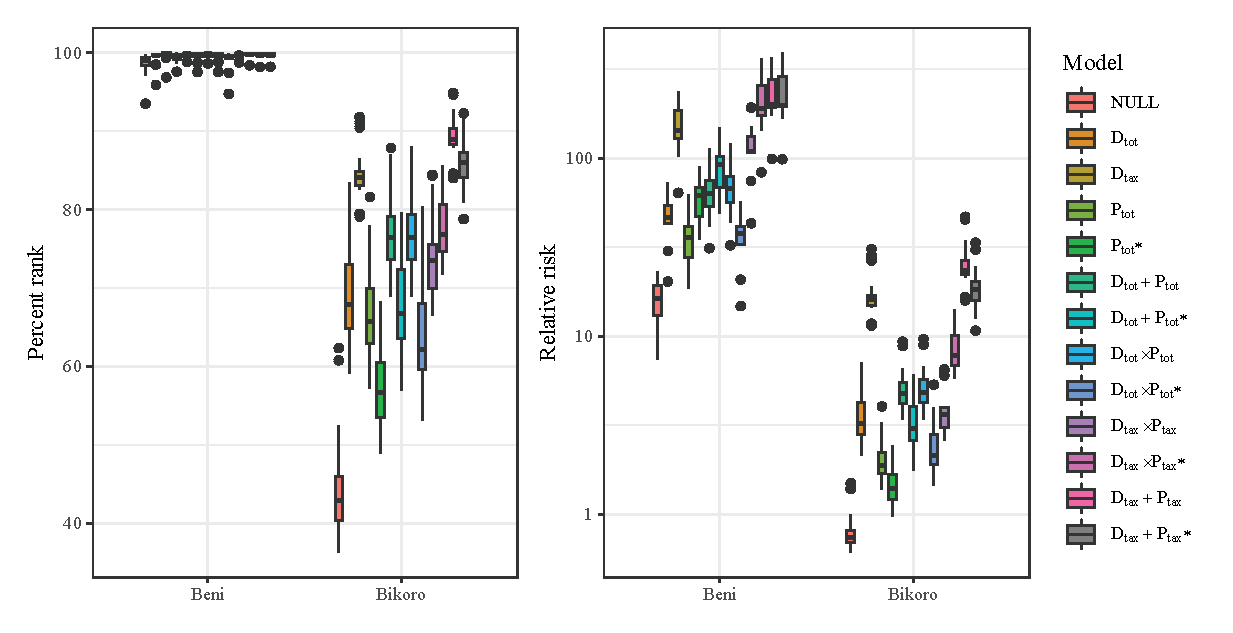
\includegraphics[width=.95\linewidth]{Fig_altModelSeltection.eps}
		\caption{\textbf{Model prediction comparison} All proposed models predictive scores for the cells covering the health districts in which the two most recent DRC outbreaks occurred for the month of outbreak occurrence (July and April respectively). \textit{Left:} Percent rank against all cells in all months, \textit{Right:} relative risk of \textit{Ebolavirus} spillover in to human populations. Models contain different covariate combinations of bat diversity ($D$), and bat birth terms ($B$) with were either separated by taxonomic group ($_{tax}$) or combined as ($_{tot}$). Alternative models that contain the down-weighted fruit bat term are denoted by *}
		\label{fig:F_alt selection}
	\end{figure}
	The top model for human spillover risk by qAIC used the taxonomically separated probability of birth terms and included the down-weighted fruit bat modification (*). Significant terms identified included EVD spillover into a non-human host in the month of and month prior to an outbreak, suggesting the model's sensitivity to the stuttering infection chains within the system and supporting observed patterns of infection transmission. The down-weighted probability of birthing term for the African fruit bat group 5-6 months prior, and the month of and month proceeding spillover events for both the fruit bats and non-molossid microbats were significant to predictions and top two models are summarized in Table~\ref{table:spatGLM_HUM} (See SI Table 6 for full alternative model results). Diversity of non-bat mammals was again identified as a significant predictor although neither viral detection in bats, nor the effect of forest fragmentation were identified as significant predictors of ebolavirus spillover to humans within this analysis. Risk of EVD spillover to humans was somewhat different to that of spillover into the non-human spillover hosts, as annual risk was more diffuse across Central Africa and more evenly distributed across areas of Western Africa (Fig ~\ref{fig:F_ridge_risk}). Similar to the non-human spillover hosts, the highest risk zones occurred around the border of Gabon and the RoC, although Cameroon was included and the high risk of spillover within the CAR were missing from the human model results. The associated temporal analysis (Fig.~\ref{fig:F_ridge_risk} \textit{right}) suggest seasonality within the system with two distinct periods of increased risk centered around the months of June and November just north of the equator. Acknowledging possible surveillance bias, the difference in peak relative risk between the human and non-human spillover host models suggest potential differences in spillover mechanisms between human and non-reservoir mammal host systems.\par
\begin{table}[h!]
	\centering
	\caption{Top two human Ebola virus disease risk model results\\}
	\label{table:spatGLM_HUM}	% 
	\begin{tabular}{lcccccc}
		Model: & \multicolumn{3}{c}{$D_{tax} + P_{tax*}$} & \multicolumn{3}{c}{$D_{tax} + P_{tax}$} \\
		\hline\hline
		&  Estimate & $\pm$95 CI  &  P value &  Estimate & $\pm$95 CI &  P value \\
		\hline
		Intercept) & \multicolumn{1}{r}{-30.63} & 10.04 & <0.001 & -31.62 & 10.00 & <0.001 \\
		$P_{\afb}$ & \multicolumn{1}{r}{-2.41} & 2.16 & 0.04 & -1.49 & 1.98 & 0.14 \\
		$P_{\mic}$ & \multicolumn{1}{r}{1.83} & 1.53 & 0.02 & 1.48 & 1.50 & 0.06 \\
		$P_{\mol}$ & \multicolumn{1}{r}{-0.19} & 2.00 & 0.84 & -0.45 & 2.02 & 0.66 \\
		$P_{\afb_2}$ & \multicolumn{1}{r}{0.91} & 2.04 & 0.29 & 1.39 & 1.88 & 0.15 \\
		$P_{\mic_2}$ & \multicolumn{1}{r}{-0.06} & 1.55 & 0.93 & -0.37 & 1.51 & 0.63 \\
		$P_{\mol_2}$ & \multicolumn{1}{r}{0.29} & 2.14 & 0.73 & 0.11 & 2.18 & 0.92 \\
		$P_{\afb_4}$ & \multicolumn{1}{r}{-0.39} & 1.96 & 0.9 & -0.02 & 1.84 & 0.98 \\
		$P_{\mic_4}$ & \multicolumn{1}{r}{-0.78} & 1.84 & 0.35 & -0.95 & 1.80 & 0.3 \\
		$P_{\mol_4}$ & \multicolumn{1}{r}{0.20} & 2.16 & 0.85 & 0.38 & 2.16 & 0.73 \\
		$P_{\afb_6}$ & \multicolumn{1}{r}{1.60} & 1.88 & 0.05 & 1.29 & 1.94 & 0.19 \\
		$P_{\mic_6}$ & \multicolumn{1}{r}{-0.27} & 1.61 & 0.67 & -0.23 & 1.63 & 0.78 \\
		$P_{\mol_6}$ & \multicolumn{1}{r}{1.34} & 1.98 & 0.2 & 1.48 & 1.94 & 0.13 \\
		$\Div_{\afb}$ & \multicolumn{1}{r}{2.87} & 1.59 & <0.001 & 2.88 & 1.63 & <0.001 \\
		$\Div_{\mic}$ & \multicolumn{1}{r}{1.86} & 2.76 & 0.18 & 1.92 & 2.78 & 0.18 \\
		$\Div_{\mol}$ & \multicolumn{1}{r}{-0.59} & 1.57 & 0.46 & -0.63 & 1.57 & 0.43 \\
		$\mathrm{PopDen}$ & \multicolumn{1}{r}{-0.23} & 0.25 & 0.07 & -0.23 & 0.255 & 0.08 \\
		$\mathrm{fragIndex}$ & \multicolumn{1}{r}{-0.39} & 0.51 & 0.12 & -0.4 & 0.51 & 0.12 \\
		$\mathrm{BVD}$  & \multicolumn{1}{r}{-11.54} & 937.31 & 0.98 & -11.43 & 944.88 & 0.98 \\
		$\Div_{\mathrm{MNB}}$ & \multicolumn{1}{r}{3.23} & 2.31 & <0.001 & 3.36 & 2.33 & <0.001 \\
		$\mathrm{OB}_{\mathrm{an}}$ & \multicolumn{1}{r}{4.56} & 1.57 & <0.001 & 4.5 & 1.58 & <0.001 \\
		$\mathrm{OB}_{\mathrm{an}_{l-1}}$ & \multicolumn{1}{r}{2.89} & 2.20 & 0.01 & 2.71 & 2.23 & 0.02 \\
		\hline
		qAIC  & \multicolumn{3}{c}{454.93} & \multicolumn{3}{c}{457.58} \\
		$\hat{c}$ & \multicolumn{3}{c}{0.78} & \multicolumn{3}{c}{0.79} \\
	\end{tabular}%
\end{table}

	The two most recent EVD outbreaks in the DRC provided a test of the predictive power of our model (Fig.~\ref{fig:F_DRC_breakdown}). The EVD outbreak announced by the WHO in July likely started in April within the Bikoro health district in the northeastern part of the country close to the border with RoC \cite{Barry2018}. This health district showed seasonality with peaks and troughs in the relative risk of viral spillover into humans (Fig.~\ref{fig:F_DRC_breakdown}). Of the 16 cells that covered the Bikoro health district there was a median percent rank scores of 88.3\% compared to all cells in all months. Relative risk of ebolavirus spillover fluctuated between minimum, median, and high of 14.9, 21.3 and 50.4 respectively. The more recent EVD outbreak occurred in the district of Beni, a persistently highly ranked region. The district in northwestern DRC near the border with Uganda announced the outbreak on first of August with the index case was presumably in July or June \cite{WHO2018}. The smaller region was covered by only nine cells and risk percent rank values extracted from the model covering July were among the highest ranking of all cells with a median of 99.6\%, minimum of 98.0\% and maximum of 99.8\%. Relative risk for the region was considerable with minimal values of 93.0, a median of 195.0 and a high of 273 across the year. Percent rank and relative risk scores were very similar between $D + B_{tax}*$ and  $D + B_{tax}$ models with the later preforming slightly better in both metrics at the Bikoro site. We ultimately chose the  $D + B_{tax}*$ model as our top model due to it's inclusion of more precise information related to our \textit{a priori} hypotheses, and its comparable predictive power over all other alternative models.
	%%
	\section*{Discussion}
	The spatial and temporal occurrence of ebolavirus on the landscape is complex, with seasonal drivers likely modifying the behaviors of both the (yet unidentified) maintenance reservoir host(s) and susceptible non-maintenance host populations. The inability of outbreak investigation teams to determine a definitive source of infection in all but a small number of cases has severely hindered the ability of public health officials to generate actionable measures against future EVD outbreak events. Infections from non-human spillover hosts to humans have only been confirmed from great apes and duikers, despite ebolavirus sequence detection in some Rodentia species \cite{Morvan1999}, Chiropteran species and the wide diversity of susceptible species within the biome \cite{Leroy2004,Swanepoel1996}. Here we predict the continental birthing patterns of African bats and find some statistical support for bats births, and African fruit bats in particular, being correlated with EVD outbreaks. Together we use these to predict the spatio-temporal risk of EVD outbreaks in non-human mammals and humans across the African continent. \par
	\begin{figure}[h!]
		\centering
		\includegraphics[width=.95\linewidth]{Fig_spilloverRiskRidge.eps}
		\caption{\textbf{Risk of Ebola virus disease outbreaks among people} Left: Mean annual risk of EVD emergence in humans across the study area. Low values are in yellow, high values in red, and grey zones were not included in the analysis. \textit{Right:} Risk of EVD aggregated by latitude and month. Height and color intensity are proportional to the risk of EVD within the latitudinal window.}
		\label{fig:F_ridge_risk}
	\end{figure}

	The natural history, distributions and diversity of African bat species are broad yet through this analysis we are able to generate the first comprehensive spatio-temporal predictions for bat parturition events. Data availability ultimately required the use of several simplifying assumptions, most notably the consolidation of species into the taxonomic groups. This simplification creates scenarios in which within a single location two taxonomic members can give birth at different, non-overlapping times during a single birth pulse, or that a single species at two separate locations can give birth at different times again within a broader birth pulse. Despite this, the patterns predicted were largely consistent with previous work \cite{Cumming1997} with only minor deviations. The reduction in predictive signal from a biannual, or continual birthing above 10$^{\circ}$ is novel, although potentially an artefact of scare data availability at the northern most latitudes of our study extent. Our analysis also refined the latitudinal threshold from polyestrous to monoestrous from the 18$^{\circ}$S to 10$^{\circ}$S and was supported by more observations than the northern phenomenon. Data mining and collection highlighted the spatial and taxonomic bias of observations with extremely limited data availability for some of the largest, densest forests in continental Africa, and low representation of the most diverse taxonomic groups. However, models with terms describing the birth pulses of bats preformed highly for both the human and non-reservoir spillover host spatGLM. Furthermore the inclusion of the proportionally down-weighted birth term for the African fruit bats species improved predictive ability in most cases.\par 
	The discovery of statistical support for some African fruit bats species being correlated with ebolavirus outbreaks supports a number of previously disparate hypotheses \cite{Hayman2015, Walsh2005, Han2016}. The historical association of EVD spillover events and African fruit bats has been more anecdotal than factual in most cases, and to date no hunters targeting fruit bats have been confirmed index cases despite the widespread practice \cite{Kamins2011,Mickleburgh2009,Peel2017}. This may be because the species most hunted, \textit{Eidolon helvum} \cite{Kamins2011, Mickleburgh2009}, is likely not a reservoir species, possibly due in part to its single annual birth pulse (in contrast to some other African fruit bats species) \cite{Hayman2012, Hayman2010} and unique cellular mechanisms \cite{ng2015}. The large geographic spread by viral subtypes, such as that observed in the 2014 outbreak in West Africa, could be facilitated by other broad ranging African fruit bats such as the hammer-headed bat, whose population spans both Central to West African regions with little measurable population genetic structure \cite{Hassanin2016}. Until recently the only potential reservoir species from which EVD-causing Ebola virus viral fragments have been recovered were Pteropodidae members \cite{Leroy2005, Olival2014}. Serological surveys have implicated molossid and non-molossid species, however serological data are difficult to interpret \cite{gilbert2013}. Our analysis also identified molossid birthing events as a potential contributor to human risk of EVD spillover and both serological and molecular findings are consistent with the patterns observed in MARV infected \textit{R. aegyptiacus} \cite{Pourrut2009, Amman2012}. Recent detections of ebolavirus fragments in molossid species and our analyses suggest the role of molossid bats in ebolavirus sylvatic maintenance is an important area for potential research \cite{Kupferschmidt2019, Goldstein2018}.\par
	Seasonality of EVD events has been noted \cite{Schmidt2017}, however the abiotic conditions (such as rainfall) used within these analyses are likely not directly driving spillover, especially for unstable RNA viruses in tropical environments \cite{Fischer2015}. We hypothesized viral persistence within bat populations themselves, meaning viral sylvatic dynamics, are also unlikely to be directly attributable to exogenous pressures. By exchanging the traditional abiotic metrics of seasonality with a derived metric such as seasonality of birth we are able to explore a mechanistically plausible driver of seasonality within the sylvatic EVD system \cite{Altizer2006} and aim to understand both necessary and sufficient causes of EVD emergence and contributions of bats as reservoirs \cite{nishiura2009find,rothman1976causes}. Temporally varying bat birth terms identified by both our non-human spillover host and human risk models support the hypothesis that birthing may facilitate transmission into non-human mammals \cite{Pourrut2009,Schuh2017}. In our best models for ebolavirus spillover the birthing term for both fruit bats and non-molossid microbats were significant. The later of the lag terms identified for the African fruit bats is consistent with the maternally derived anti-body (MDA) hypothesis of Pourrut \textit{et al.} \cite{Pourrut2009} and Peel \textit{et al.} \cite{Peel2018}, dynamics predicted by generic filovirus models \cite{Hayman2015}, and observed in empirical MARV data \cite{Amman2012}. \par
	Risk of spillover to non-human spillover hosts was strongly driven by human population density and responsible for much of the patchy geographic risk distribution (see SI Figure 4). This negative human population density-EVD risk relationship was still significant but effect size was much smaller within the human system. This may be expected given many outbreaks in animals are identified in forest-dwelling species, such as gorillas, and concurrently with human cases where index cases are reported to have had contact with other species such as gorillas \cite{Leroy2004}. The correlation of non-bat mammalian diversity in both spillover models could indicate simply that both the bat hosts and the non-reservoir spillover hosts live in the biodiverse tropical forests. Temporally lagged terms that describe chains of infection, both from bats to non-humans spillover hosts and from them to humans, were significant in our models as expected. In contrast to other work, however, we did not find habitat fragmentation to be predictive of EVD spillover risk \cite{Rulli2017}, perhaps because we are not modeling changes in forest through time or because we are modeling risk at a much larger scale than those studies (but see also \cite{Wilkinson2018}) and thus Simpson's paradox applies, using slightly different methods, or because the other terms in our models are more important. It is difficult to consider how instances of Simpson's paradox may be influencing our results, but clearly the interactions between habitat change, bat birthing, ebolavirus emergence and disease emergence in general are areas for future research \cite{Rulli2017, Wilkinson2018, Han2016}. Data sets to test these relationships, such as one populated with animal infections independent of human outbreak events, however, present serious hurdles in these regards. \par
	\begin{figure}[h!]
		\centering
		\includegraphics[width=.95\linewidth]{DRCoutbreak.eps}
		\caption{\textbf{Model results in the context of the most recent EVD outbreaks} In 2018 there were two recognized EVD outbreaks in the Democratic Republic of the Congo (DRC).The district of Bikoro where the July 2018 outbreak occurred is highlighted in blue, and highlighted in orange is the district of Beni where the outbreak announced in August 2018 started. The index case for the Bikoro epidemic was believed to be in April, while the Beni outbreak is believed to have begun in July. \textit{Upper:} Percent risk ranking against all cells and all months (not just the DRC). \textit{Lower:} Relative risk of viral spillover. \textit{Left:} Annual average risk by district health zone. \textit{Right:} Risk with in the health districts throughout the year. Each lines represents a cell within the district and the median value is bolded.}
		\label{fig:F_DRC_breakdown}
	\end{figure}
	The DRC has seen more EVD outbreak events than any other country, and the two most recent outbreaks exemplify the country's ongoing struggle to combat a complex system. While the seasonality of relative risk is largely similar between the two locations, there are distinct and potentially important local peaks and troughs within the local seasonality of risk for each location and both outbreaks occurred at, or close to, local maximal values of relative risk. These seasonal patterns may be linked to the biannual birth pulses of the local fruit bat or molossid species, but are also likely tied to extremely local shifts in behavioral, phenological, and climatic factors that modify both the reservoir host(s) and susceptible populations.\par
	Analyses of EVD emergence, including ours, are clearly limited by sparse data. This includes information on other possible host species such as apes, swine and other small mammals, which may warrant further investigation if data become available. Most recent serological analyses of African primates, however, support our assumptions that they are unlikely to be maintenance hosts \cite{ayouba2019,hayman2019}. The lack of detailed species specific bat birthing data hampered our ability to test some hypotheses and necessitated the aggregation of data by host taxonomic traits rather than a species, or genus level. While these groupings have proved useful \cite{Cumming1997}, we do acknowledge that the patterns discussed may not be fully representative for all members (i.e. \textit{E. helvum}) and was our primary motivation for creating down-weighted variation. However, despite individual bat variations, our model still broadly captures when species such as \textit{E. helvum} give birth in space and time, even if the particular species only gives birth annually \cite{Peel2017}. Despite the significance of only fruit bat associated diversity terms, non-molossid microbats are under sampled virologically \cite{Leendertz2016} and ecologically (this study) for such a diverse taxonomic group. Increased data may change our understanding of their role in EVD, especially in light of the recent news of ebolavirus viral fragments in the \textit{Miniopterus inflatus} microbat and isolation of a potentially new \textit{Ebolavius} species by Goldstein \textit{et al.} \cite{Goldstein2018} from a molossid species, demonstrate the undiscovered viral diversity within the system. 
	We were also unable to include bat abundance terms, and clearly host abundance will affect the likelihood of viral persistence in populations \cite{Hayman2015, Pourrut2009}. These ecological gaps, however, can be filled without additional virological work, although contemporaneous ecological and virological data collection will provide advantages for data integration and improved system understanding \cite{Rulli2017,Pourrut2009,Amman2012, Restif2012}. Because of the limited number of viral detections, all \textit{Ebolavirus} species were combined into a generic definition of ebolavirus despite the probably that each species has its own intricacies of sylvatic persistence, distribution, reservoir host and spillover. Further, the reliance on symptomatic EVD has increased these biases if viruses had different pathological consequences in man. Only increased virological studies in hosts and unfortunately outbreaks in people will allow us to disentangle these species level intricacies. Despite these weaknesses, we believe we have successfully captured the overall patterns of birth pulses of African bats and provide potentially useful insights in the ecology of ebolaviruses and how seasonal changes in EVD risk may be driven by bat reservoir host ecology.\par

	\section*{Competing Interests}
	We have no competing interests
	
	\section*{Author Contributions}
	D.T.S.H. conceived the study;
	D.T.S.H., C.R.H., J.C.M. developed the methods;
	C.R.H. \& A.M. compiled the data;
	C.R.H. \& J.C.M. wrote the code;
	C.R.H. ran the analysis;
	A.M. provided critiques;
	C.R.H. wrote the first draft with all authors editing and reviewing the manuscript.
	
	\section*{Acknowledgements}
	We would like to acknowledge Dr. David Wilkinson for all his help, along with the many reviewers who helped.
	
	\section*{Funding}
	D.T.S.H would like to acknowledge funding by Rutherford Discovery Fellowship RDF-MAU1701 and Marsden MAU1503.
	
	%References
	\bibliography{bib_FS}
	
\end{document}
